\documentclass[10pt]{article}

\usepackage[margin=1in]{geometry}
% https://tex.stackexchange.com/questions/27802/set-noindent-for-entire-file
\setlength\parindent{0pt}
% https://tex.stackexchange.com/questions/9550/why-does-underlined-text-not-get-wrapped-once-it-hits-the-end-of-a-line
\usepackage{soul}
\usepackage{indentfirst}
\usepackage{amsmath,amsthm,amssymb,scrextend}
\DeclareMathOperator*{\argmax}{arg\,max}
\DeclareMathOperator*{\argmin}{arg\,min}
% \usepackage{fancyhdr}
% \setlength{\headheight}{14.49998pt}
% \pagestyle{fancy}
\usepackage{graphicx}

\newcommand{\cont}{\subseteq}
\usepackage{tikz}
\usepackage{pgfplots}
\pgfplotsset{width=10cm,compat=1.9}

\usepackage{amsmath}
\usepackage[mathscr]{euscript}
\let\euscr\mathscr \let\mathscr\relax
\usepackage[scr]{rsfso}
\usepackage{amsthm}
\usepackage{amssymb}
\usepackage{multicol}

\usepackage{listings}
\usepackage{xcolor}
\usepackage{float}
\definecolor{codegreen}{rgb}{0,0.6,0}
\definecolor{codegray}{rgb}{0.5,0.5,0.5}
\definecolor{codepurple}{rgb}{0.58,0,0.82}
\definecolor{backcolour}{rgb}{0.95,0.95,0.92}

\lstdefinestyle{mystyle}{
    backgroundcolor=\color{backcolour},   
    commentstyle=\color{codegreen},
    keywordstyle=\color{magenta},
    numberstyle=\tiny\color{codegray},
    stringstyle=\color{codepurple},
    basicstyle=\ttfamily\footnotesize,
    breakatwhitespace=false,         
    breaklines=true,                 
    captionpos=b,                    
    keepspaces=true,                 
    numbers=left,                    
    numbersep=5pt,                  
    showspaces=false,                
    showstringspaces=false,
    showtabs=false,                  
    tabsize=2
}

\lstset{style=mystyle}

\DeclareMathOperator{\arcsec}{arcsec}
\DeclareMathOperator{\arccot}{arccot}
\DeclareMathOperator{\arccsc}{arccsc}
\newcommand{\ddx}{\frac{d}{dx}}
\newcommand{\dfdx}{\frac{df}{dx}}
\newcommand{\ddxp}[1]{\frac{d}{dx}\left( #1 \right)}
\newcommand{\dydx}{\frac{dy}{dx}}
\let\ds\displaystyle
\newcommand{\intx}[1]{\int #1 \, dx}
\newcommand{\intt}[1]{\int #1 \, dt}
\newcommand{\defint}[3]{\int_{#1}^{#2} #3 \, dx}
\newcommand{\imp}{\Rightarrow}
\newcommand{\un}{\cup}
\newcommand{\inter}{\cap}
\newcommand{\ps}{\mathscr{P}}
\newcommand{\set}[1]{\left\{ #1 \right\}}
\newtheorem*{sol}{Solution}
\newtheorem*{claim}{Claim}
\newtheorem{problem}{Problem}
\def\mathbi#1{\textbf{\em #1}}
\begin{document}

% \lhead{Stats 303}
% \chead{Luyao Wang lw337}
% \rhead{\today}

\begin{center}
  {\Large \bf COMPSCI 308: Design and Analysis of Algorithms Homework 1}
  \vspace{2mm}

  {\bf Luyao Wang}

  {\today}
\end{center}

\section*{1. Sorting}
\subsection*{(a) Programming}

\begin{enumerate}
  \item {Implement insertion sort as a function
        \begin{verbatim}
void insertionSort(std::vector<int> &arr)
{
  int n = arr.size();

  for (int i = 1; i < n; ++i)
  {
    int key = arr[i];
    int j = i - 1;

    while (j >= 0 && arr[j] > key)
    {
      arr[j + 1] = arr[j];
      j = j - 1;
    }

    arr[j + 1] = key;
  }
}
        \end{verbatim}
        }


  \item {Implement a function of a random array with integer values of a given size n
        \begin{verbatim}
std::vector<int> generateRandomArray(int n = 10)
{
  std::random_device rd;
  std::mt19937 gen(rd());
  std::uniform_int_distribution<> dis(-INT_MIN, INT_MAX);

  std::vector<int> result(n);

  std::generate(result.begin(), result.end(), std::bind(dis, gen));

  return result;
}
        \end{verbatim}
        }
\end{enumerate}

\subsection*{(b) Analysis}

Below is the result of the experiment.

\begin{table}[H]
  \centering
  \caption{Running time for different $n$}
  \label{tab:csv_data}
  \begin{tabular}{cc}
    \hline
    \textbf{$n$} & \textbf{milliseconds} \\
    \hline
    100          & 0                     \\
    3545         & 21                    \\
    6990         & 54                    \\
    10434        & 100                   \\
    13879        & 178                   \\
    17324        & 275                   \\
    20769        & 402                   \\
    24214        & 552                   \\
    27659        & 705                   \\
    31103        & 893                   \\
    34548        & 1096                  \\
    37993        & 1321                  \\
    41438        & 1580                  \\
    44883        & 1850                  \\
    48328        & 2151                  \\
    51772        & 2520                  \\
    55217        & 2877                  \\
    58662        & 3209                  \\
    62107        & 3596                  \\
    65552        & 4093                  \\
    68997        & 4695                  \\
    72441        & 4875                  \\
    75886        & 5365                  \\
    79331        & 5897                  \\
    82776        & 6451                  \\
    86221        & 6990                  \\
    89666        & 7549                  \\
    93110        & 8312                  \\
    96555        & 8777                  \\
    100000       & 9413                  \\
    \hline
  \end{tabular}
\end{table}

Figure 1 clearly demonstrates a noticeable trend of rapidly increasing running time as the value of $n$ grows larger.

In Figure 2, I presented a plot depicting the relationship between the square root of the running time, denoted as $\sqrt{T}$, and the input size $n$. The plot reveals a linear relationship between these two variables. This outcome aligns well with the expected worst-case performance of insertion sort, which is $O(n^2)$.

\begin{figure}[H]
  \centering
  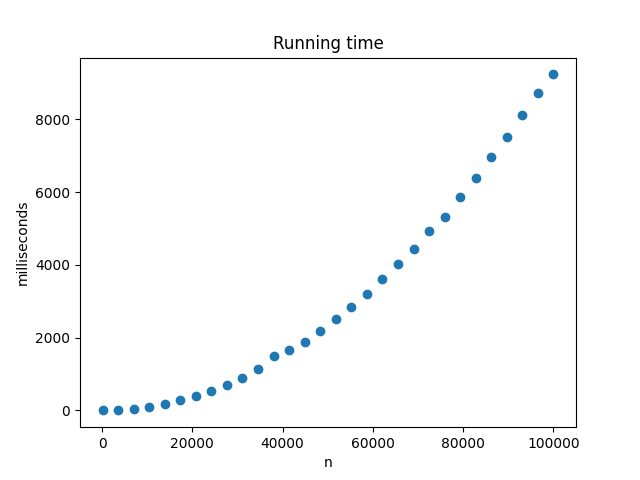
\includegraphics[width=0.8\textwidth]{../assets/runtime.png}
  \caption{Running time (milliseconds) for different $n$}
\end{figure}

\begin{figure}[H]
  \centering
  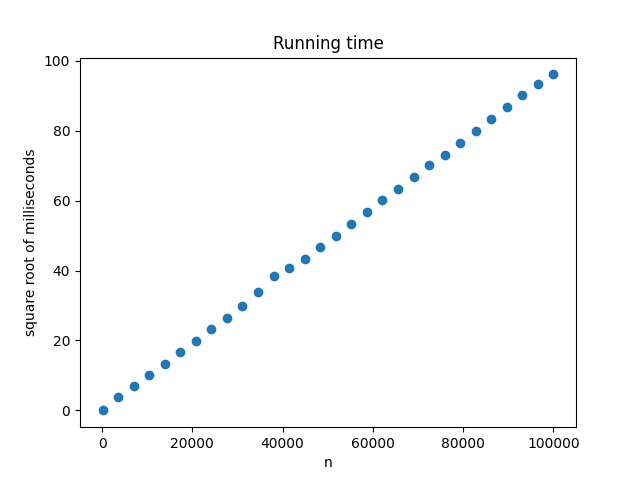
\includegraphics[width=0.8\textwidth]{../assets/squared_runtime.png}
  \caption{Square root of running time (milliseconds) for different $n$}
\end{figure}

\section*{2. Asymptotic Notations}

\begin{figure}[H]
  \centering
  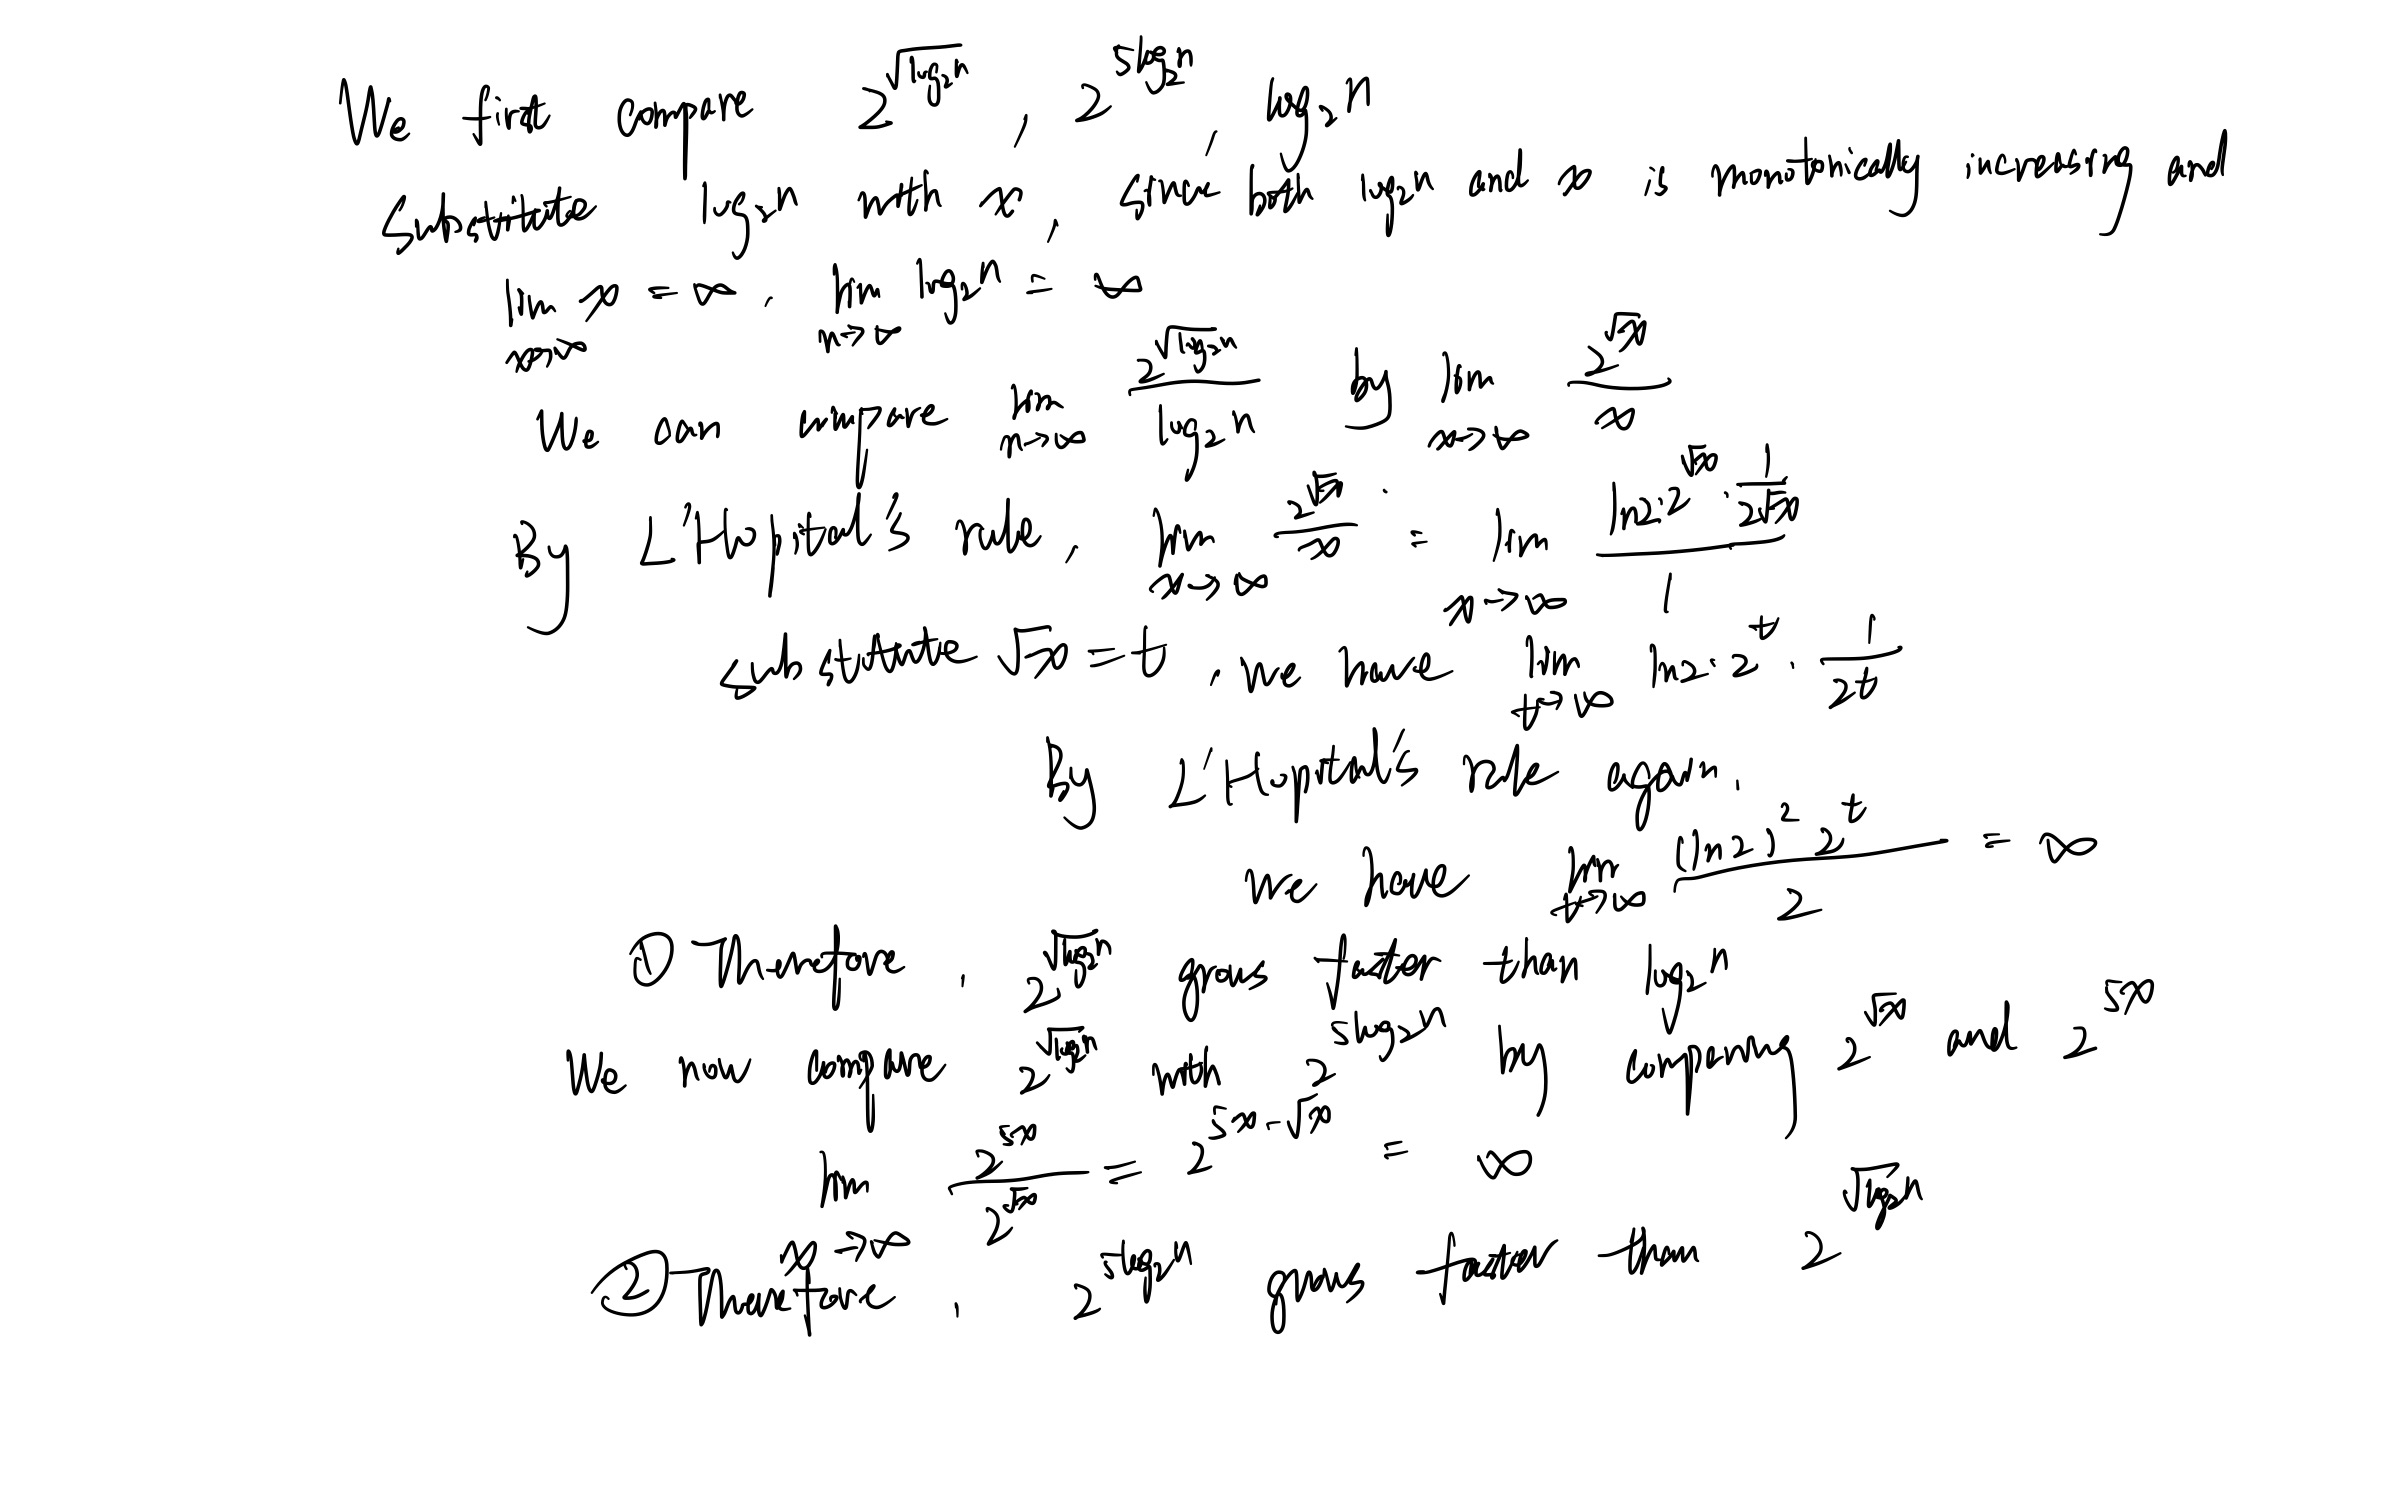
\includegraphics[width=\linewidth]{../assets/2_1.jpg}
\end{figure}

\begin{figure}[H]
  \centering
  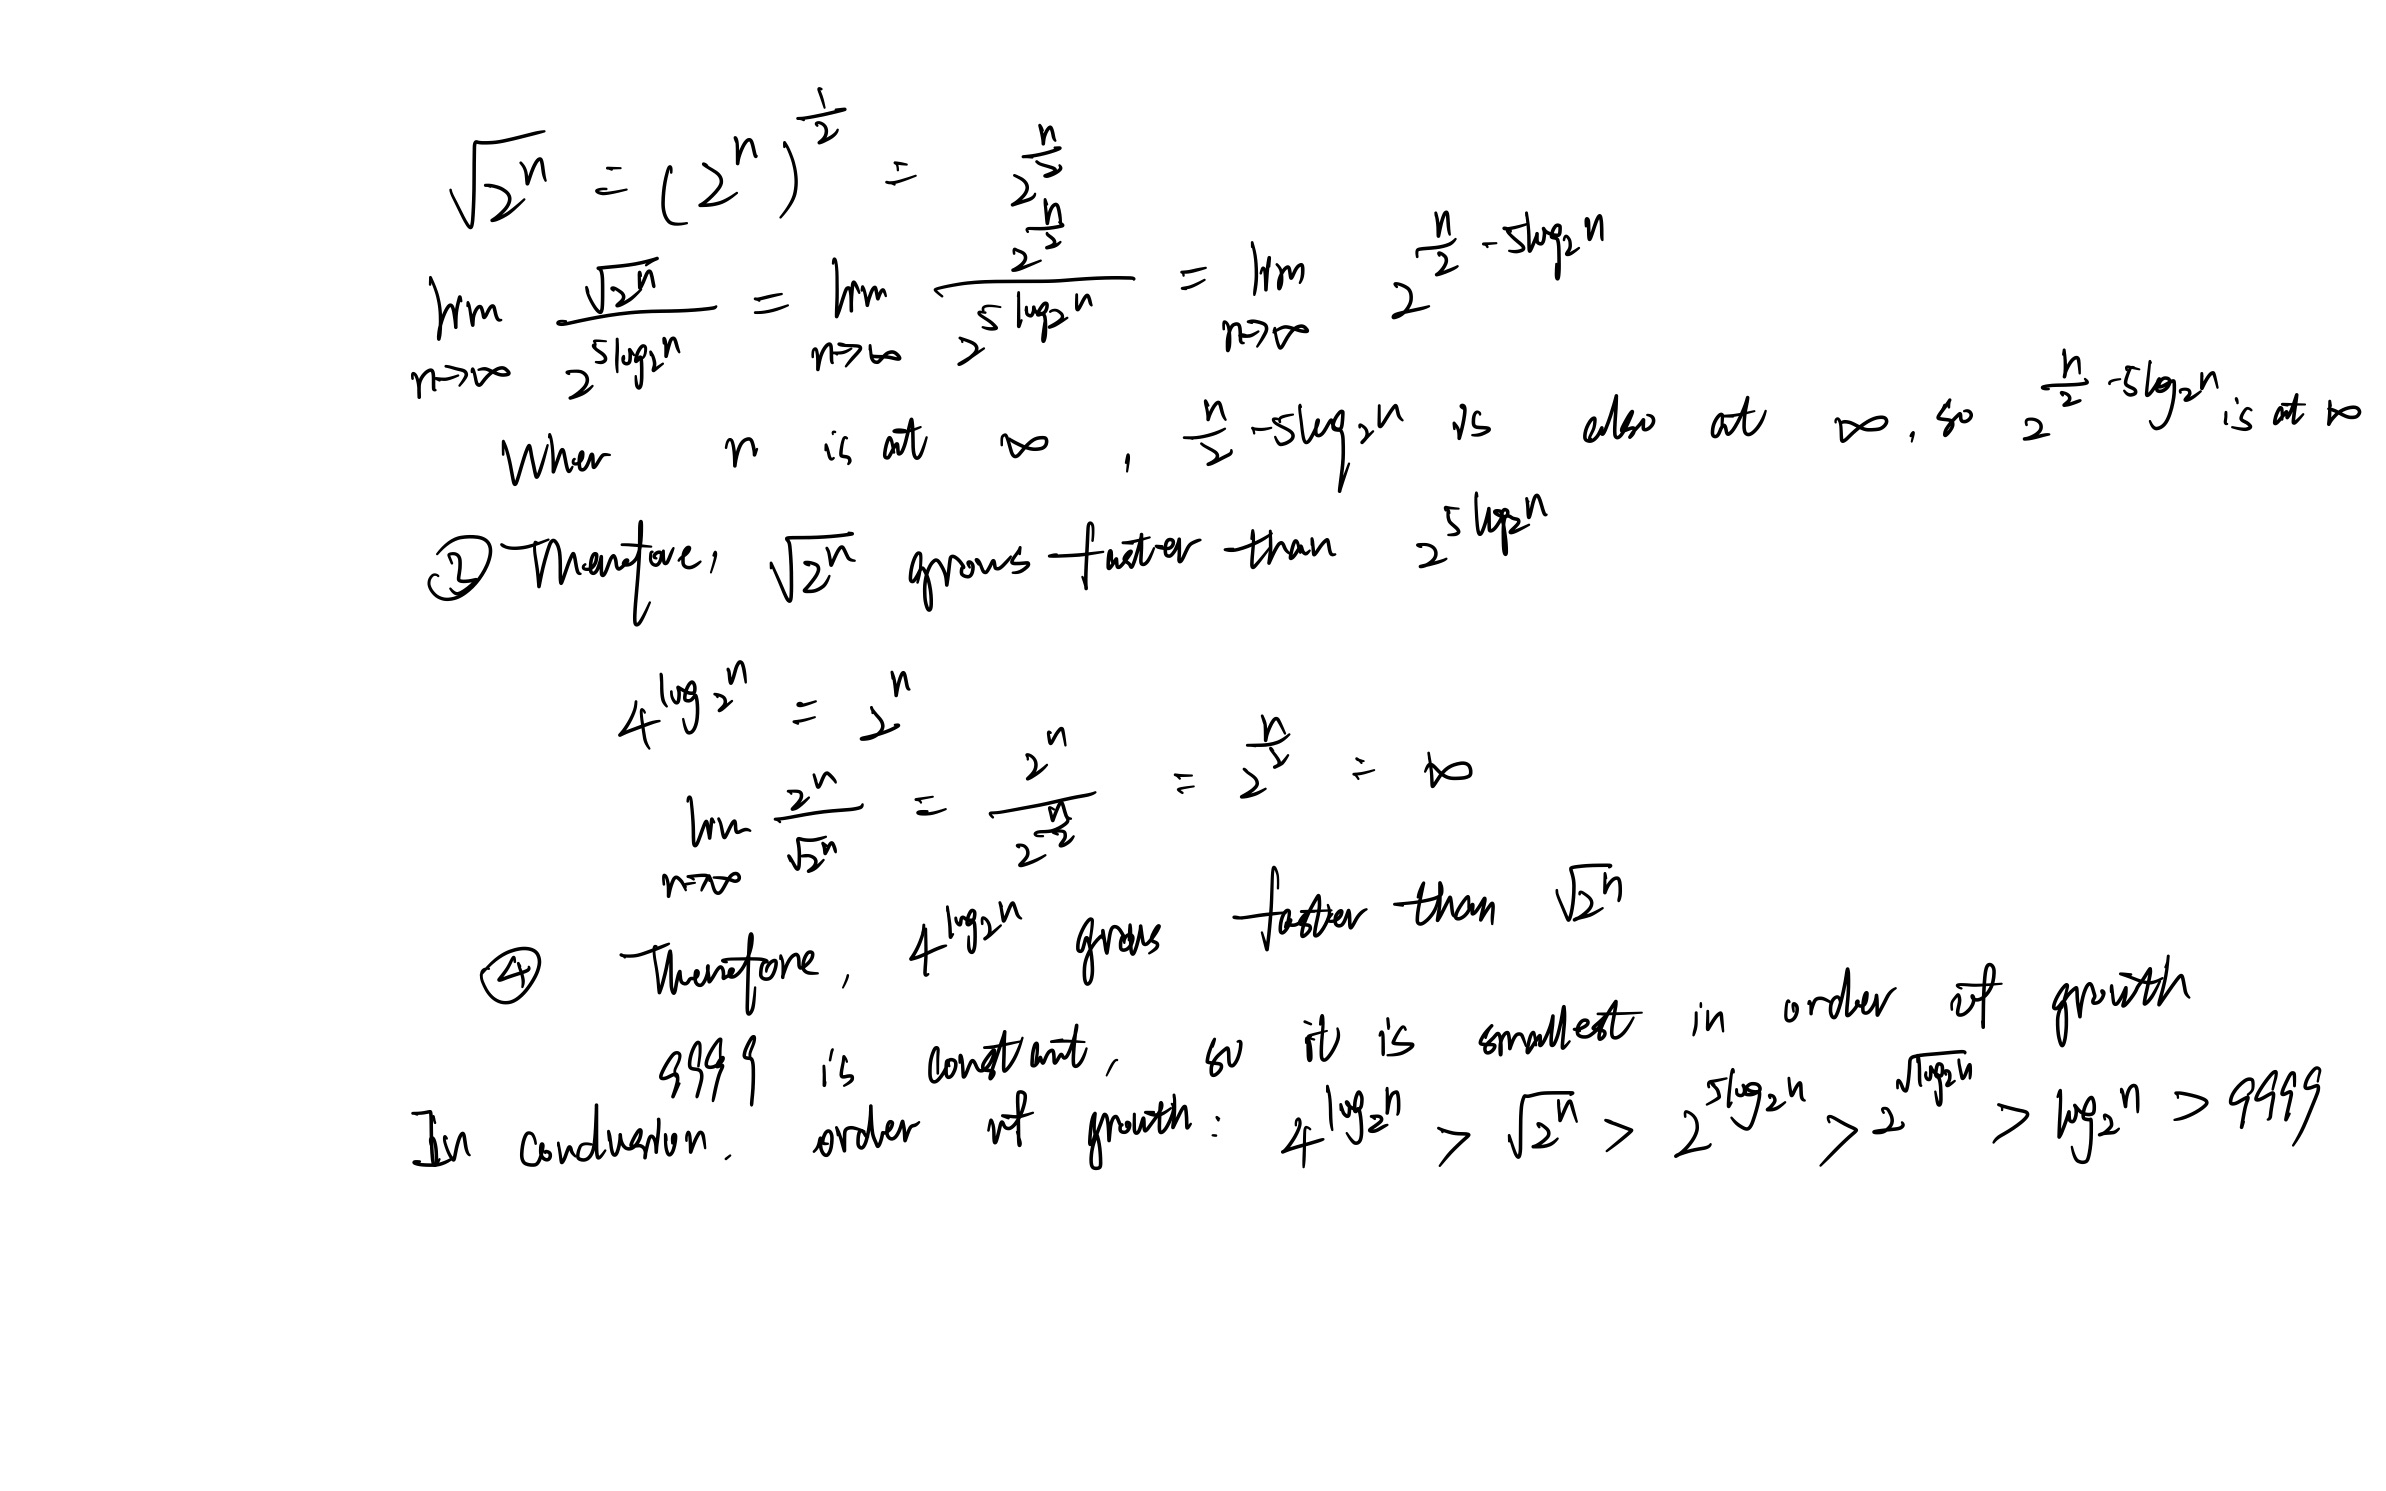
\includegraphics[width=\linewidth]{../assets/2_2.jpg}
\end{figure}

\section*{3. Proof}

\begin{figure}[H]
  \centering
  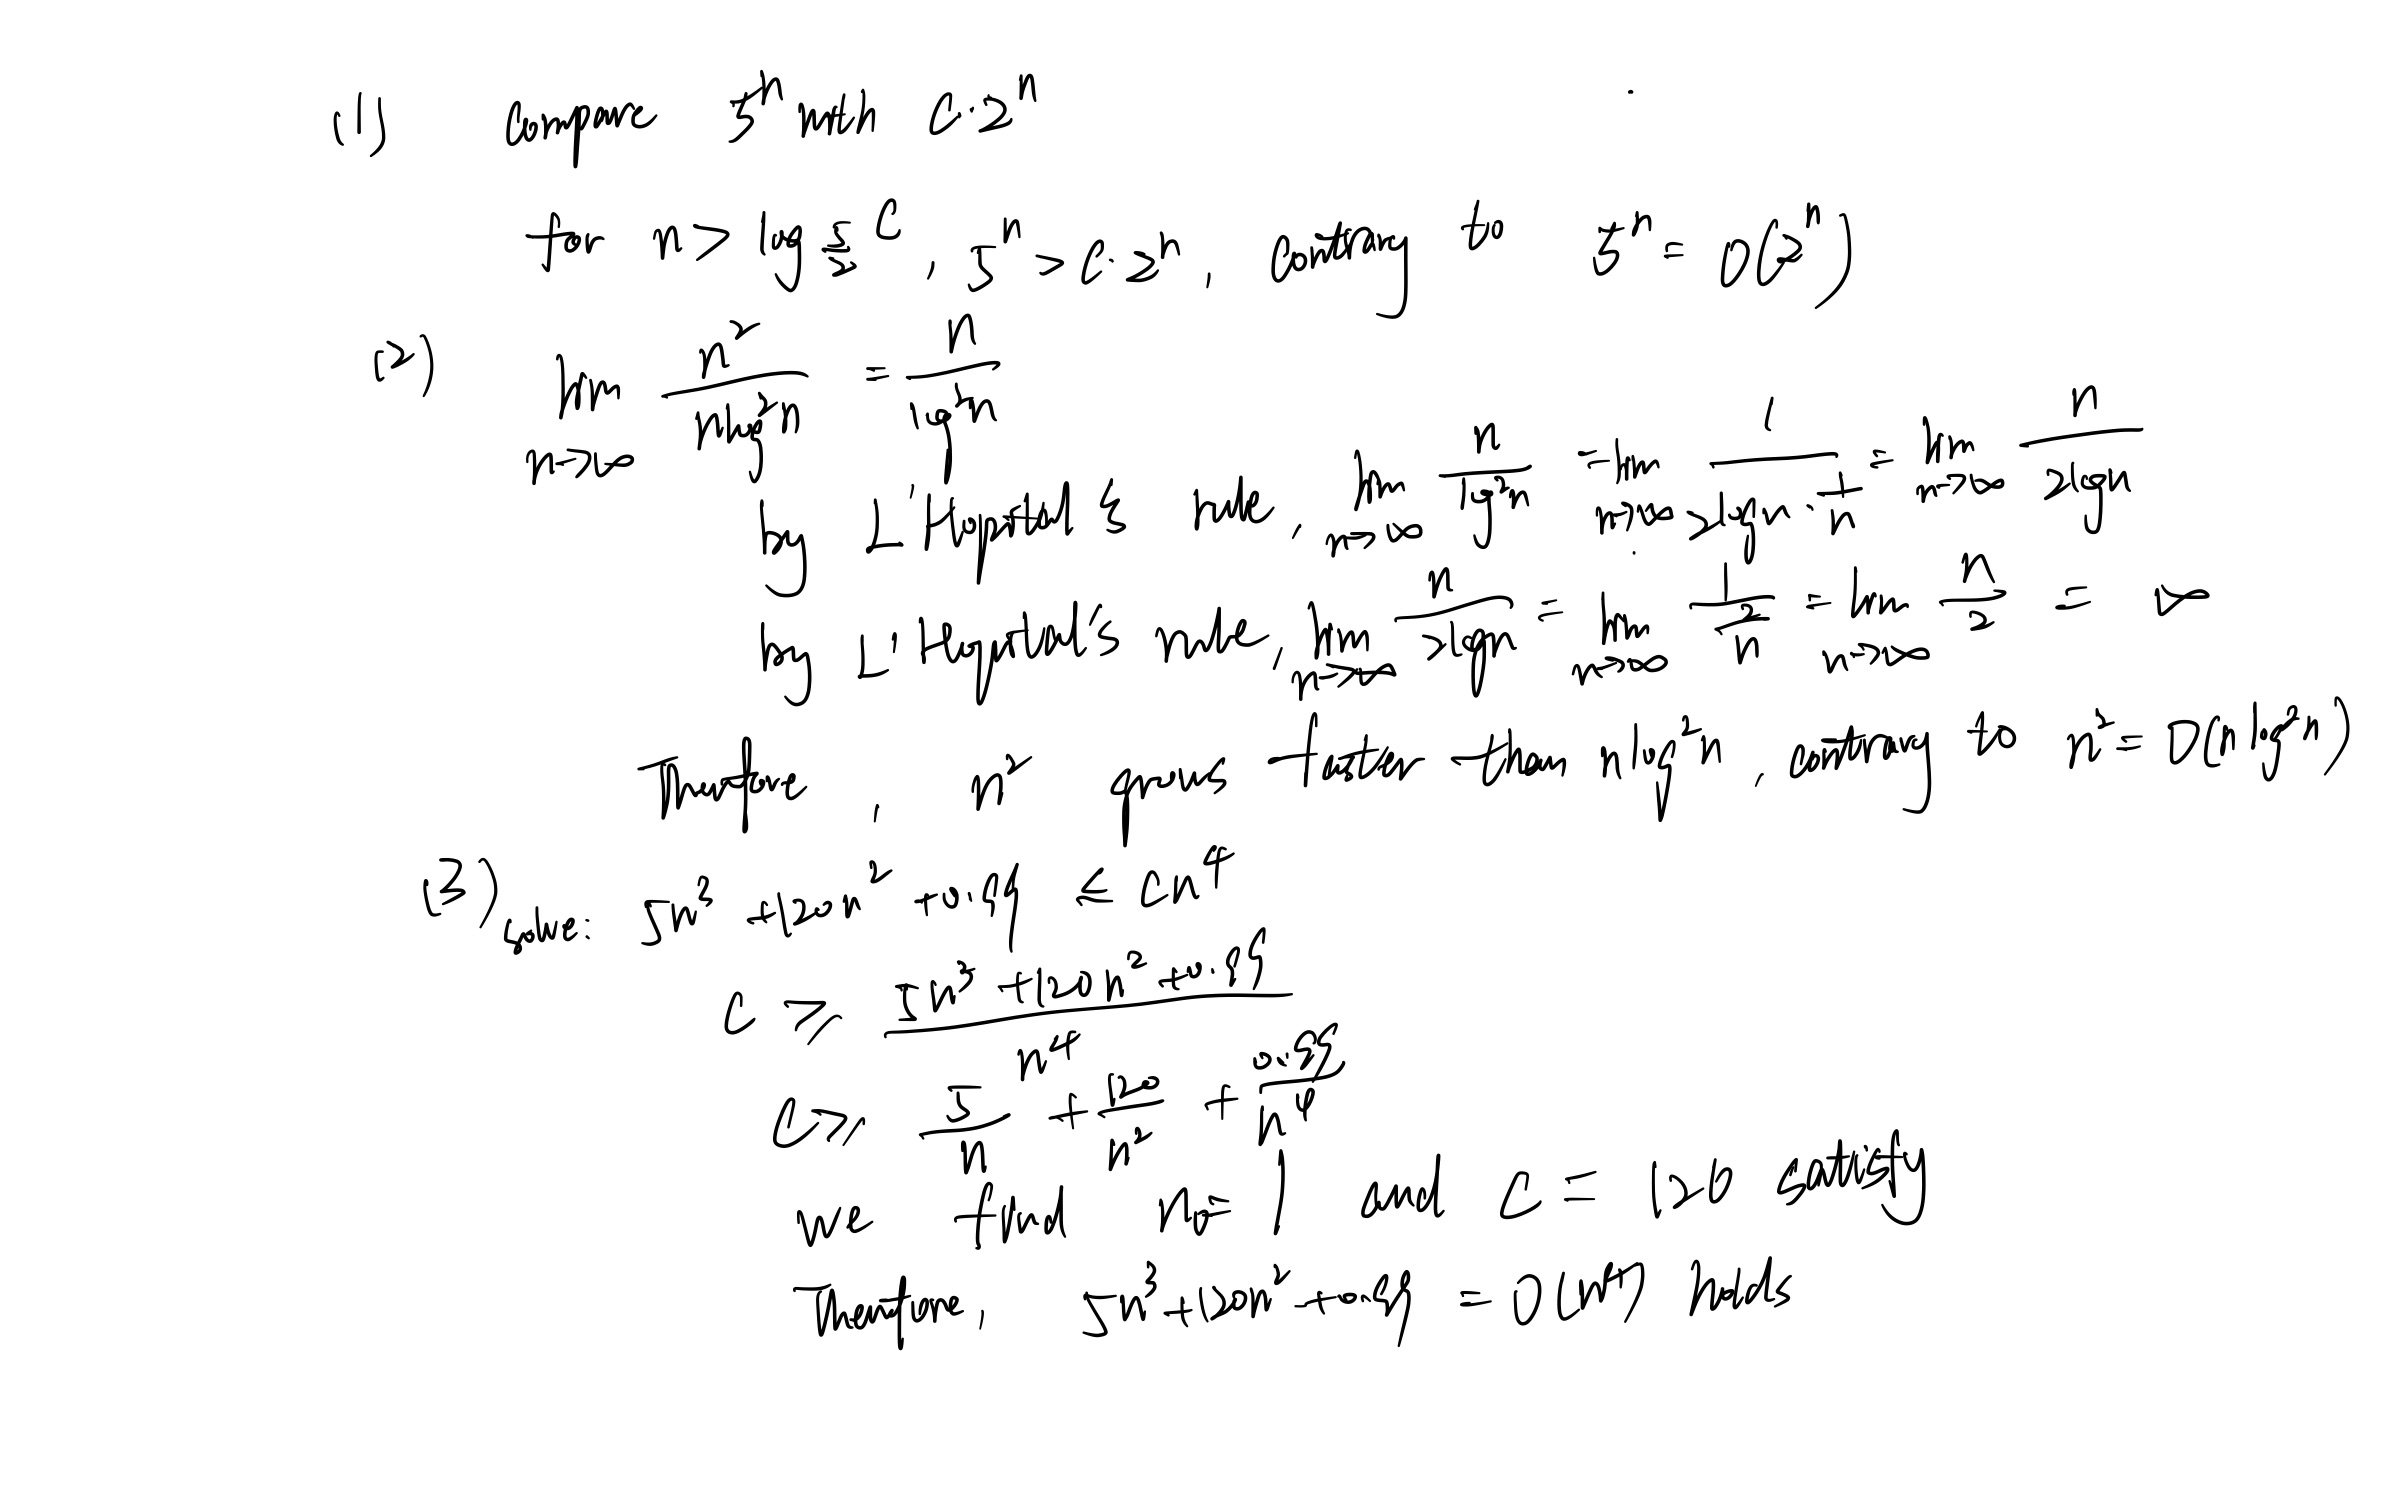
\includegraphics[width=\linewidth]{../assets/3_1.jpg}
\end{figure}

\begin{figure}[H]
  \centering
  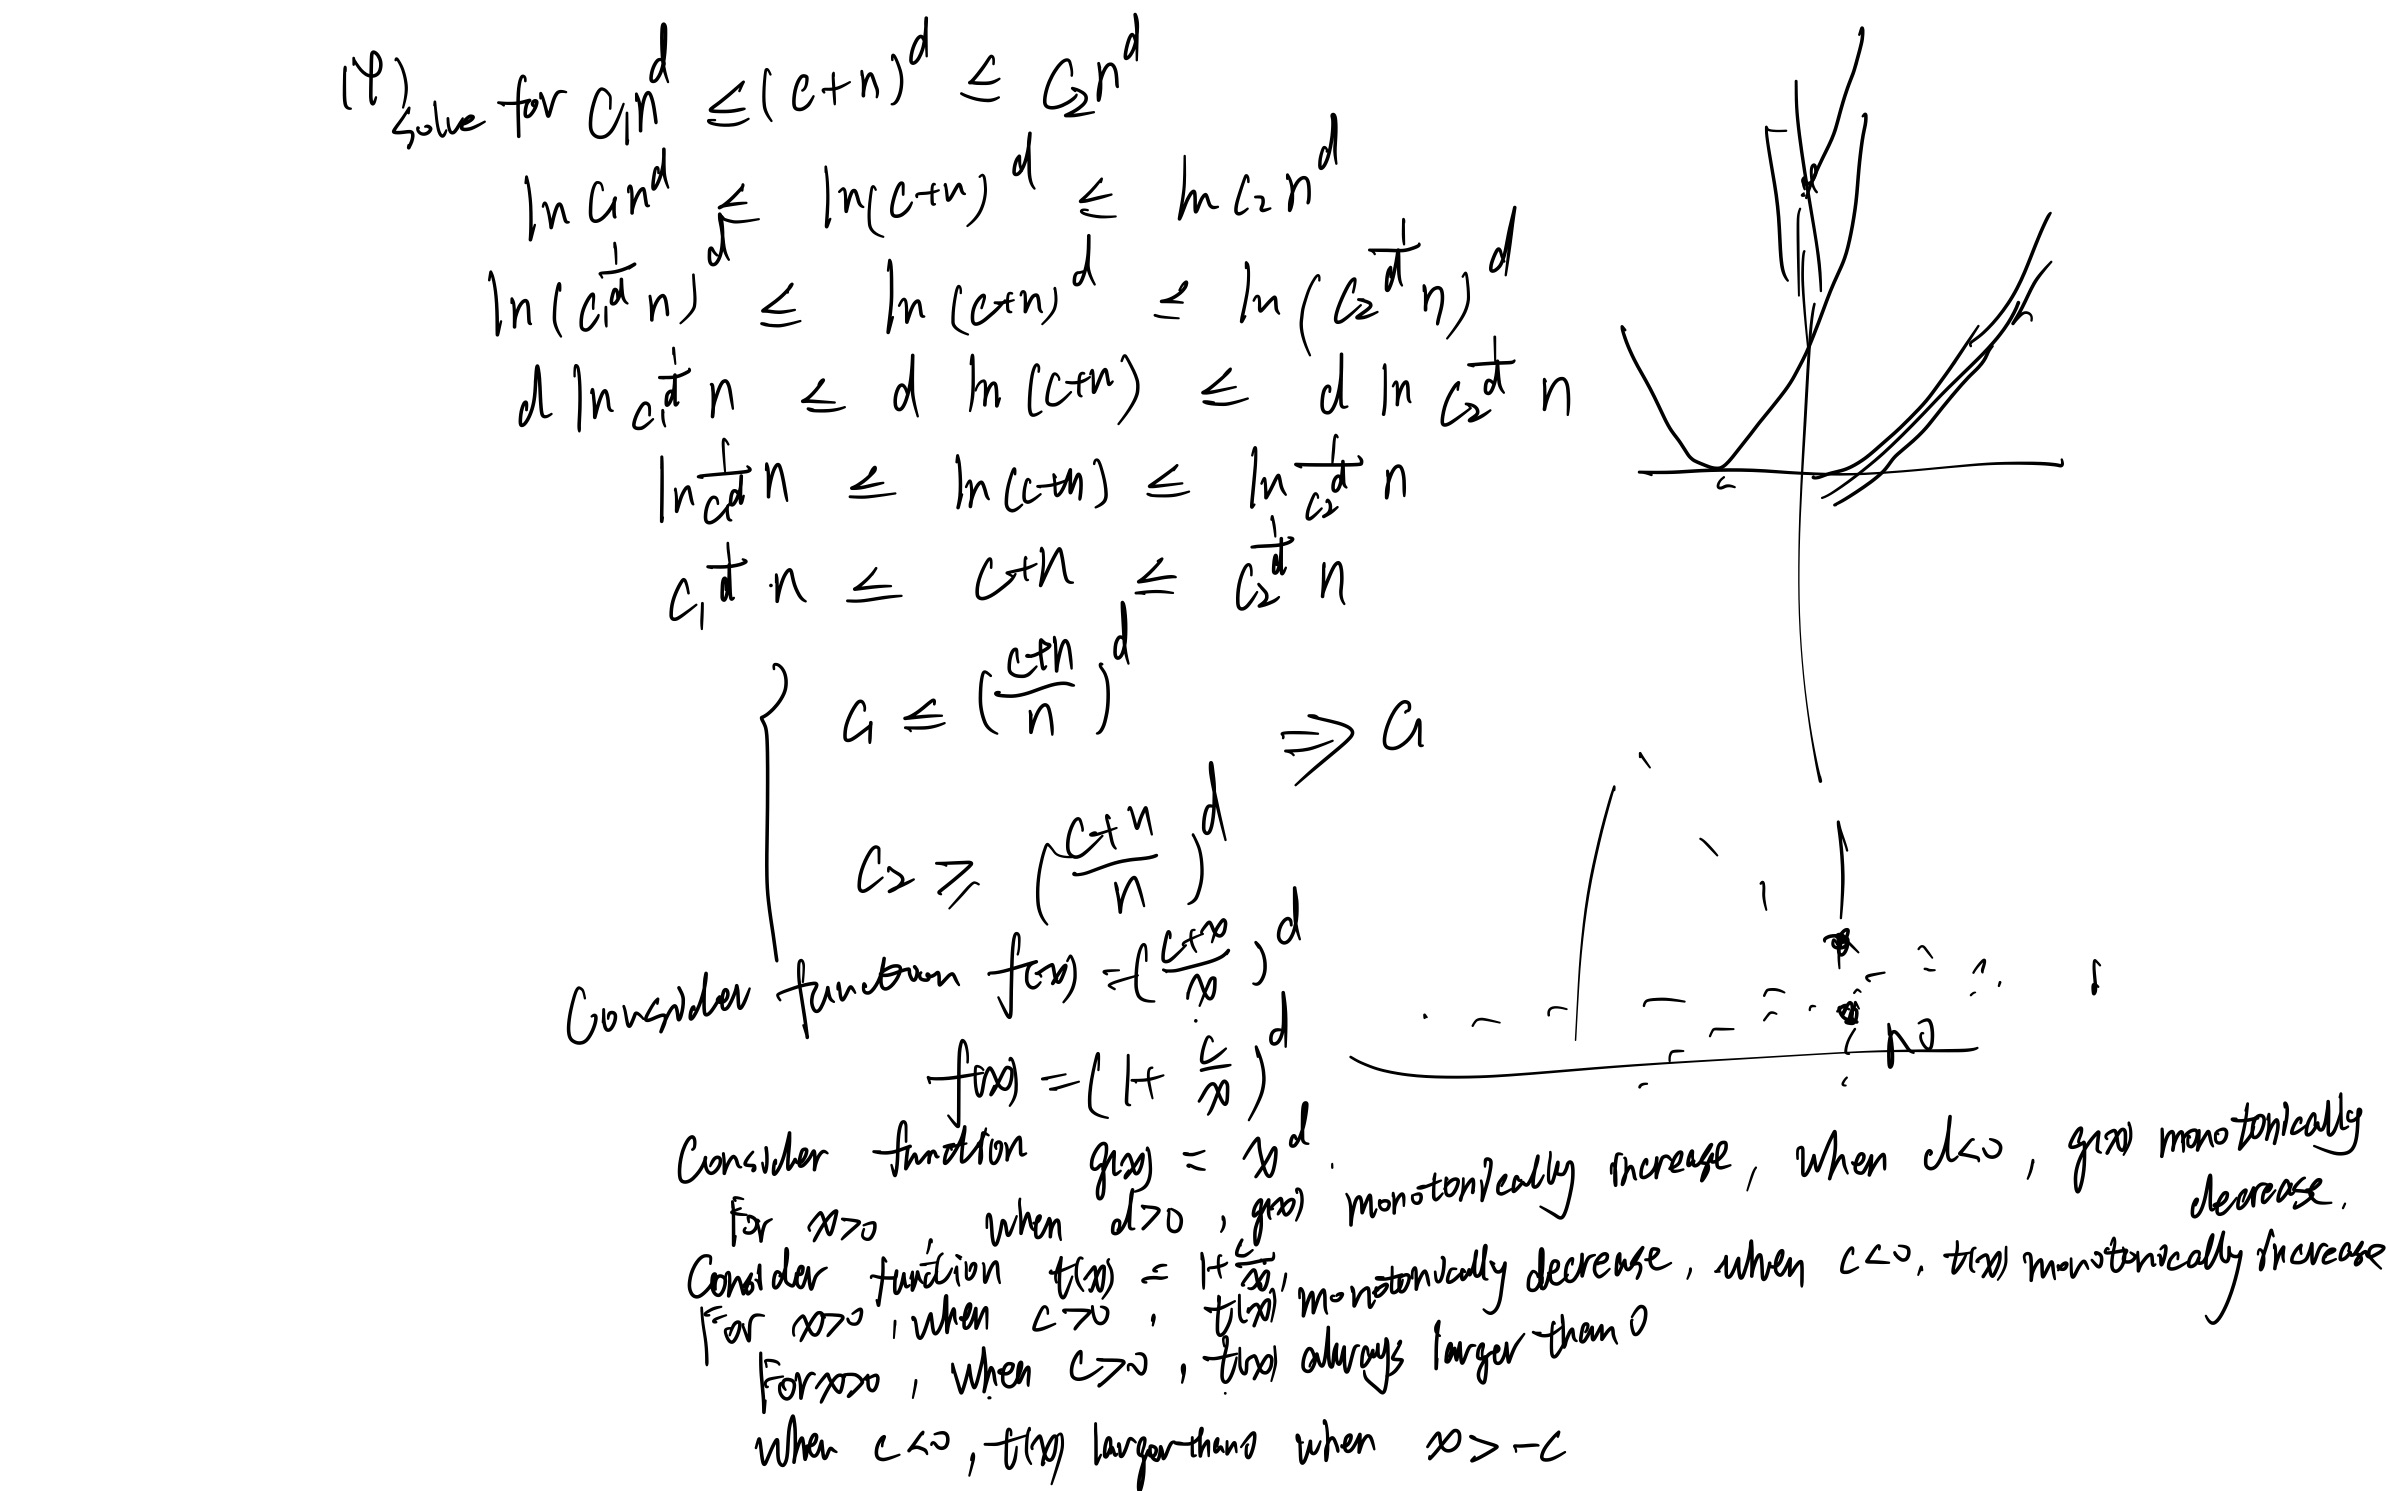
\includegraphics[width=\linewidth]{../assets/3_2.jpg}
\end{figure}

\begin{figure}[H]
  \centering
  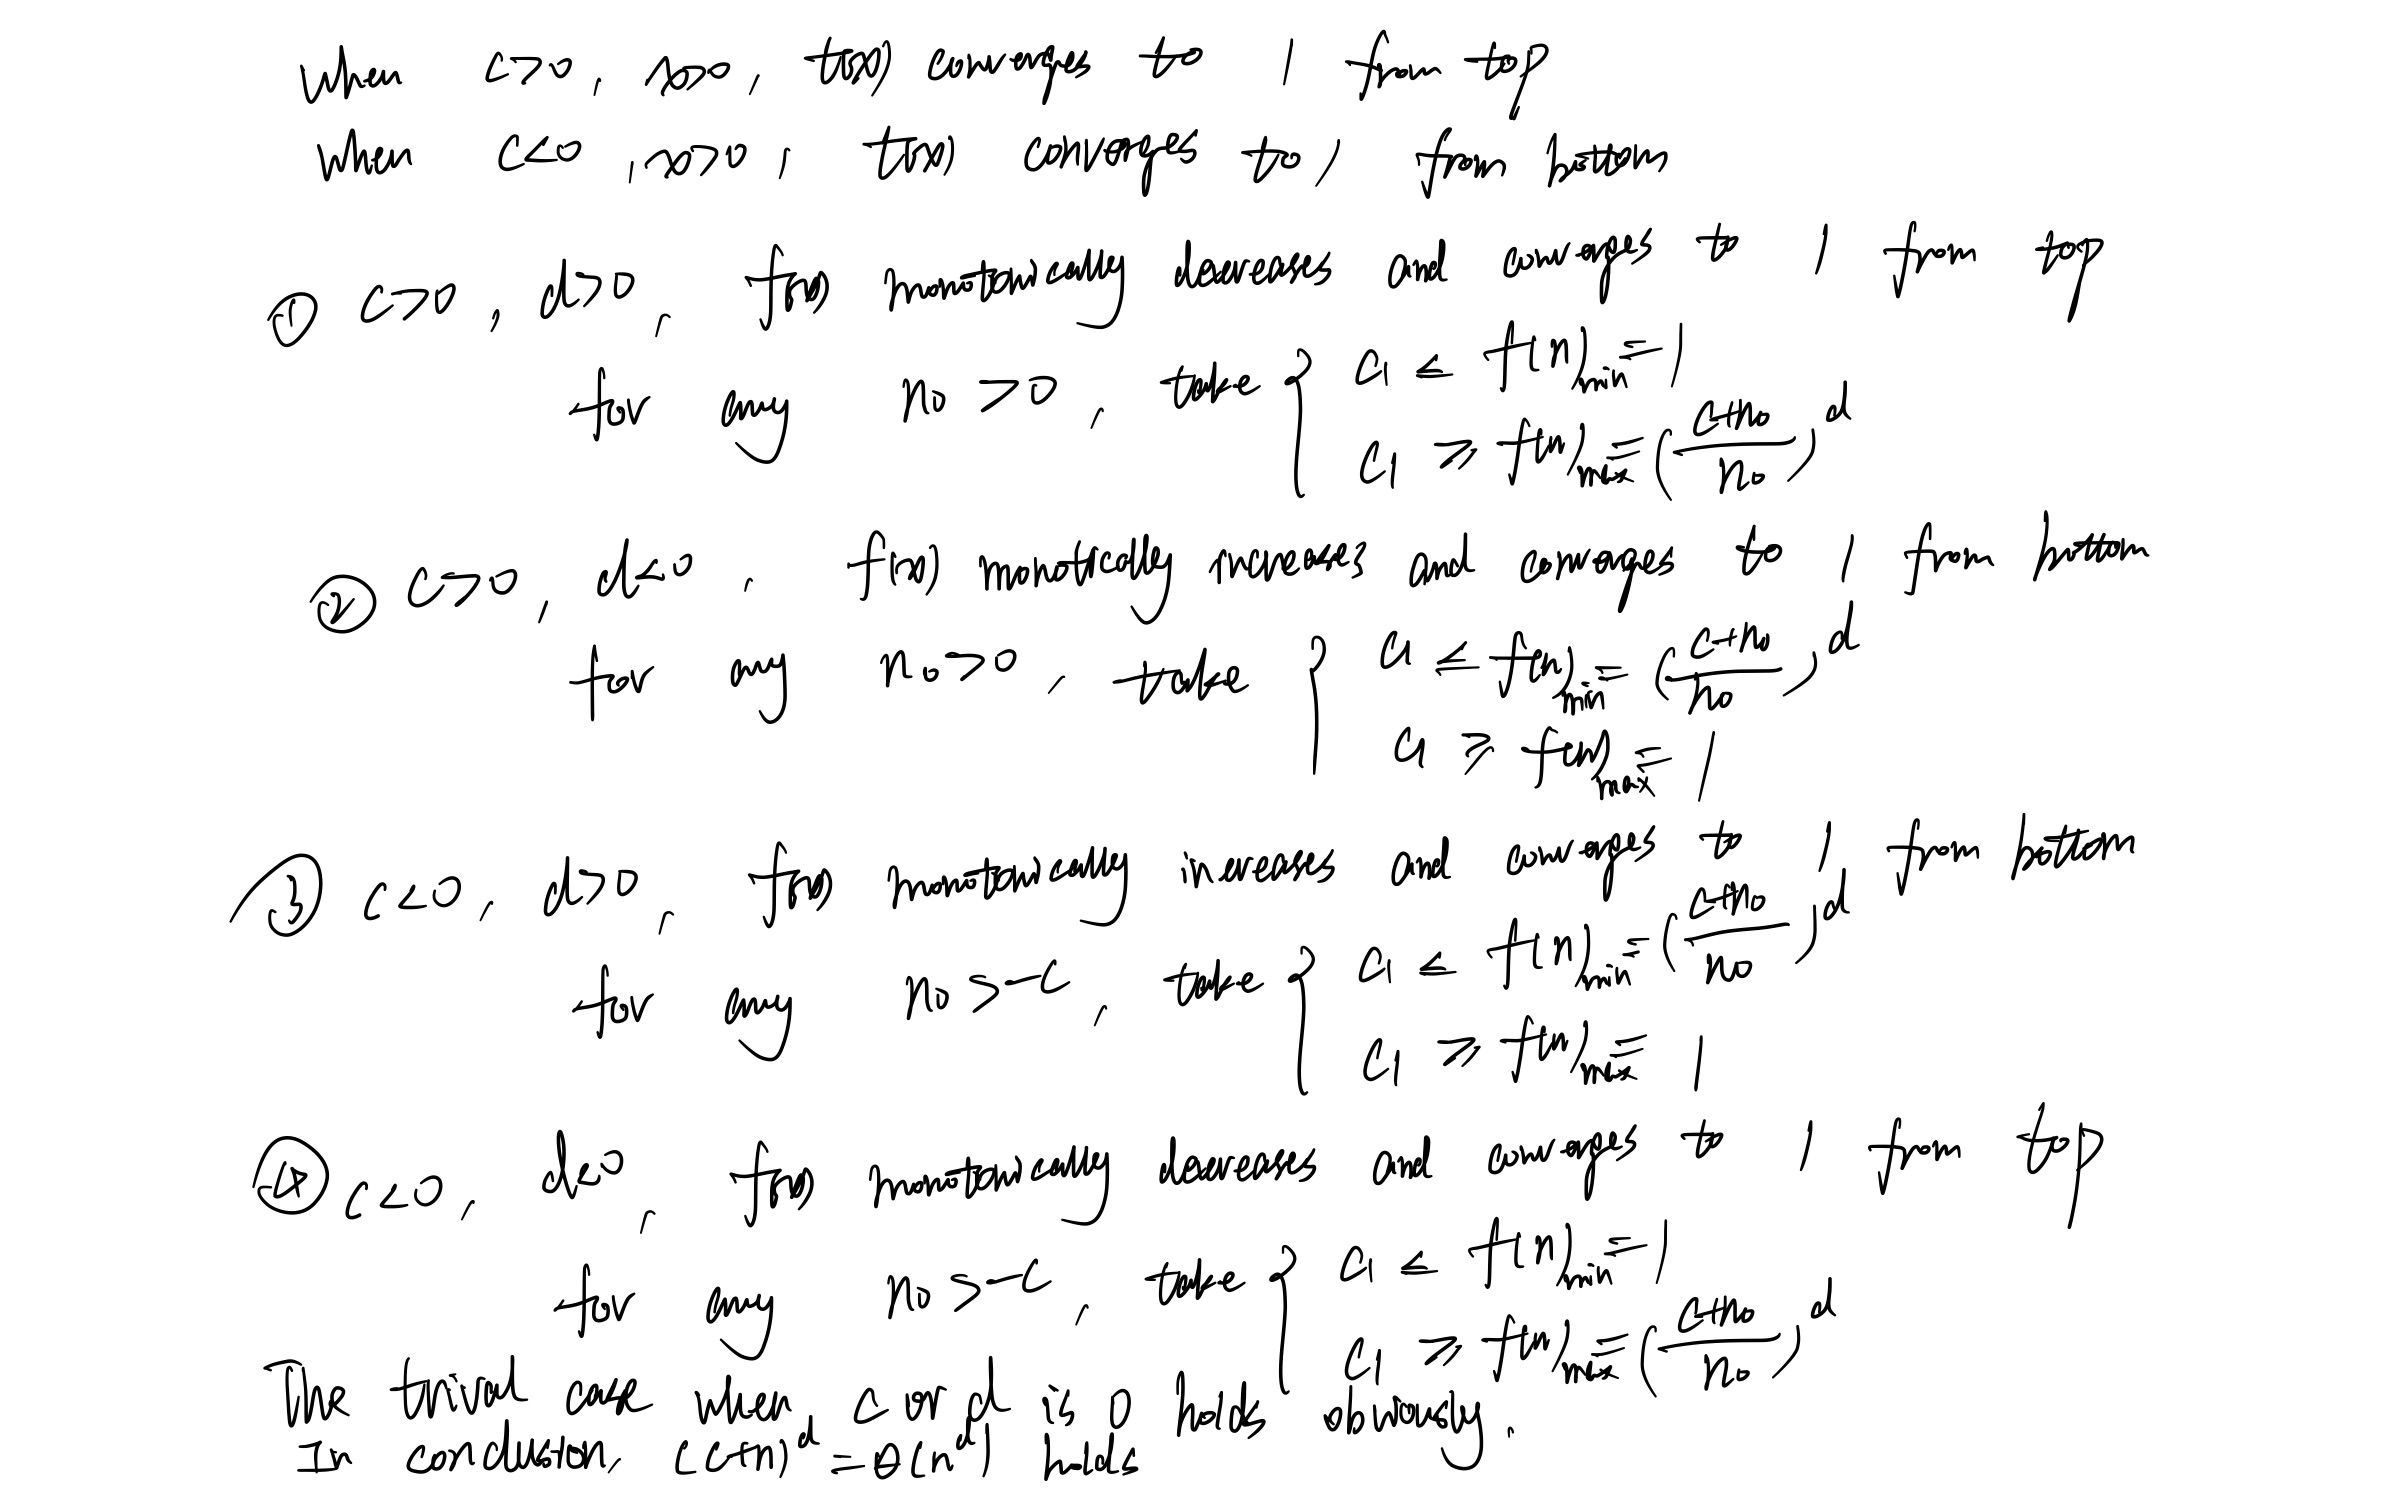
\includegraphics[width=\linewidth]{../assets/3_3.jpg}
\end{figure}

\begin{figure}[H]
  \centering
  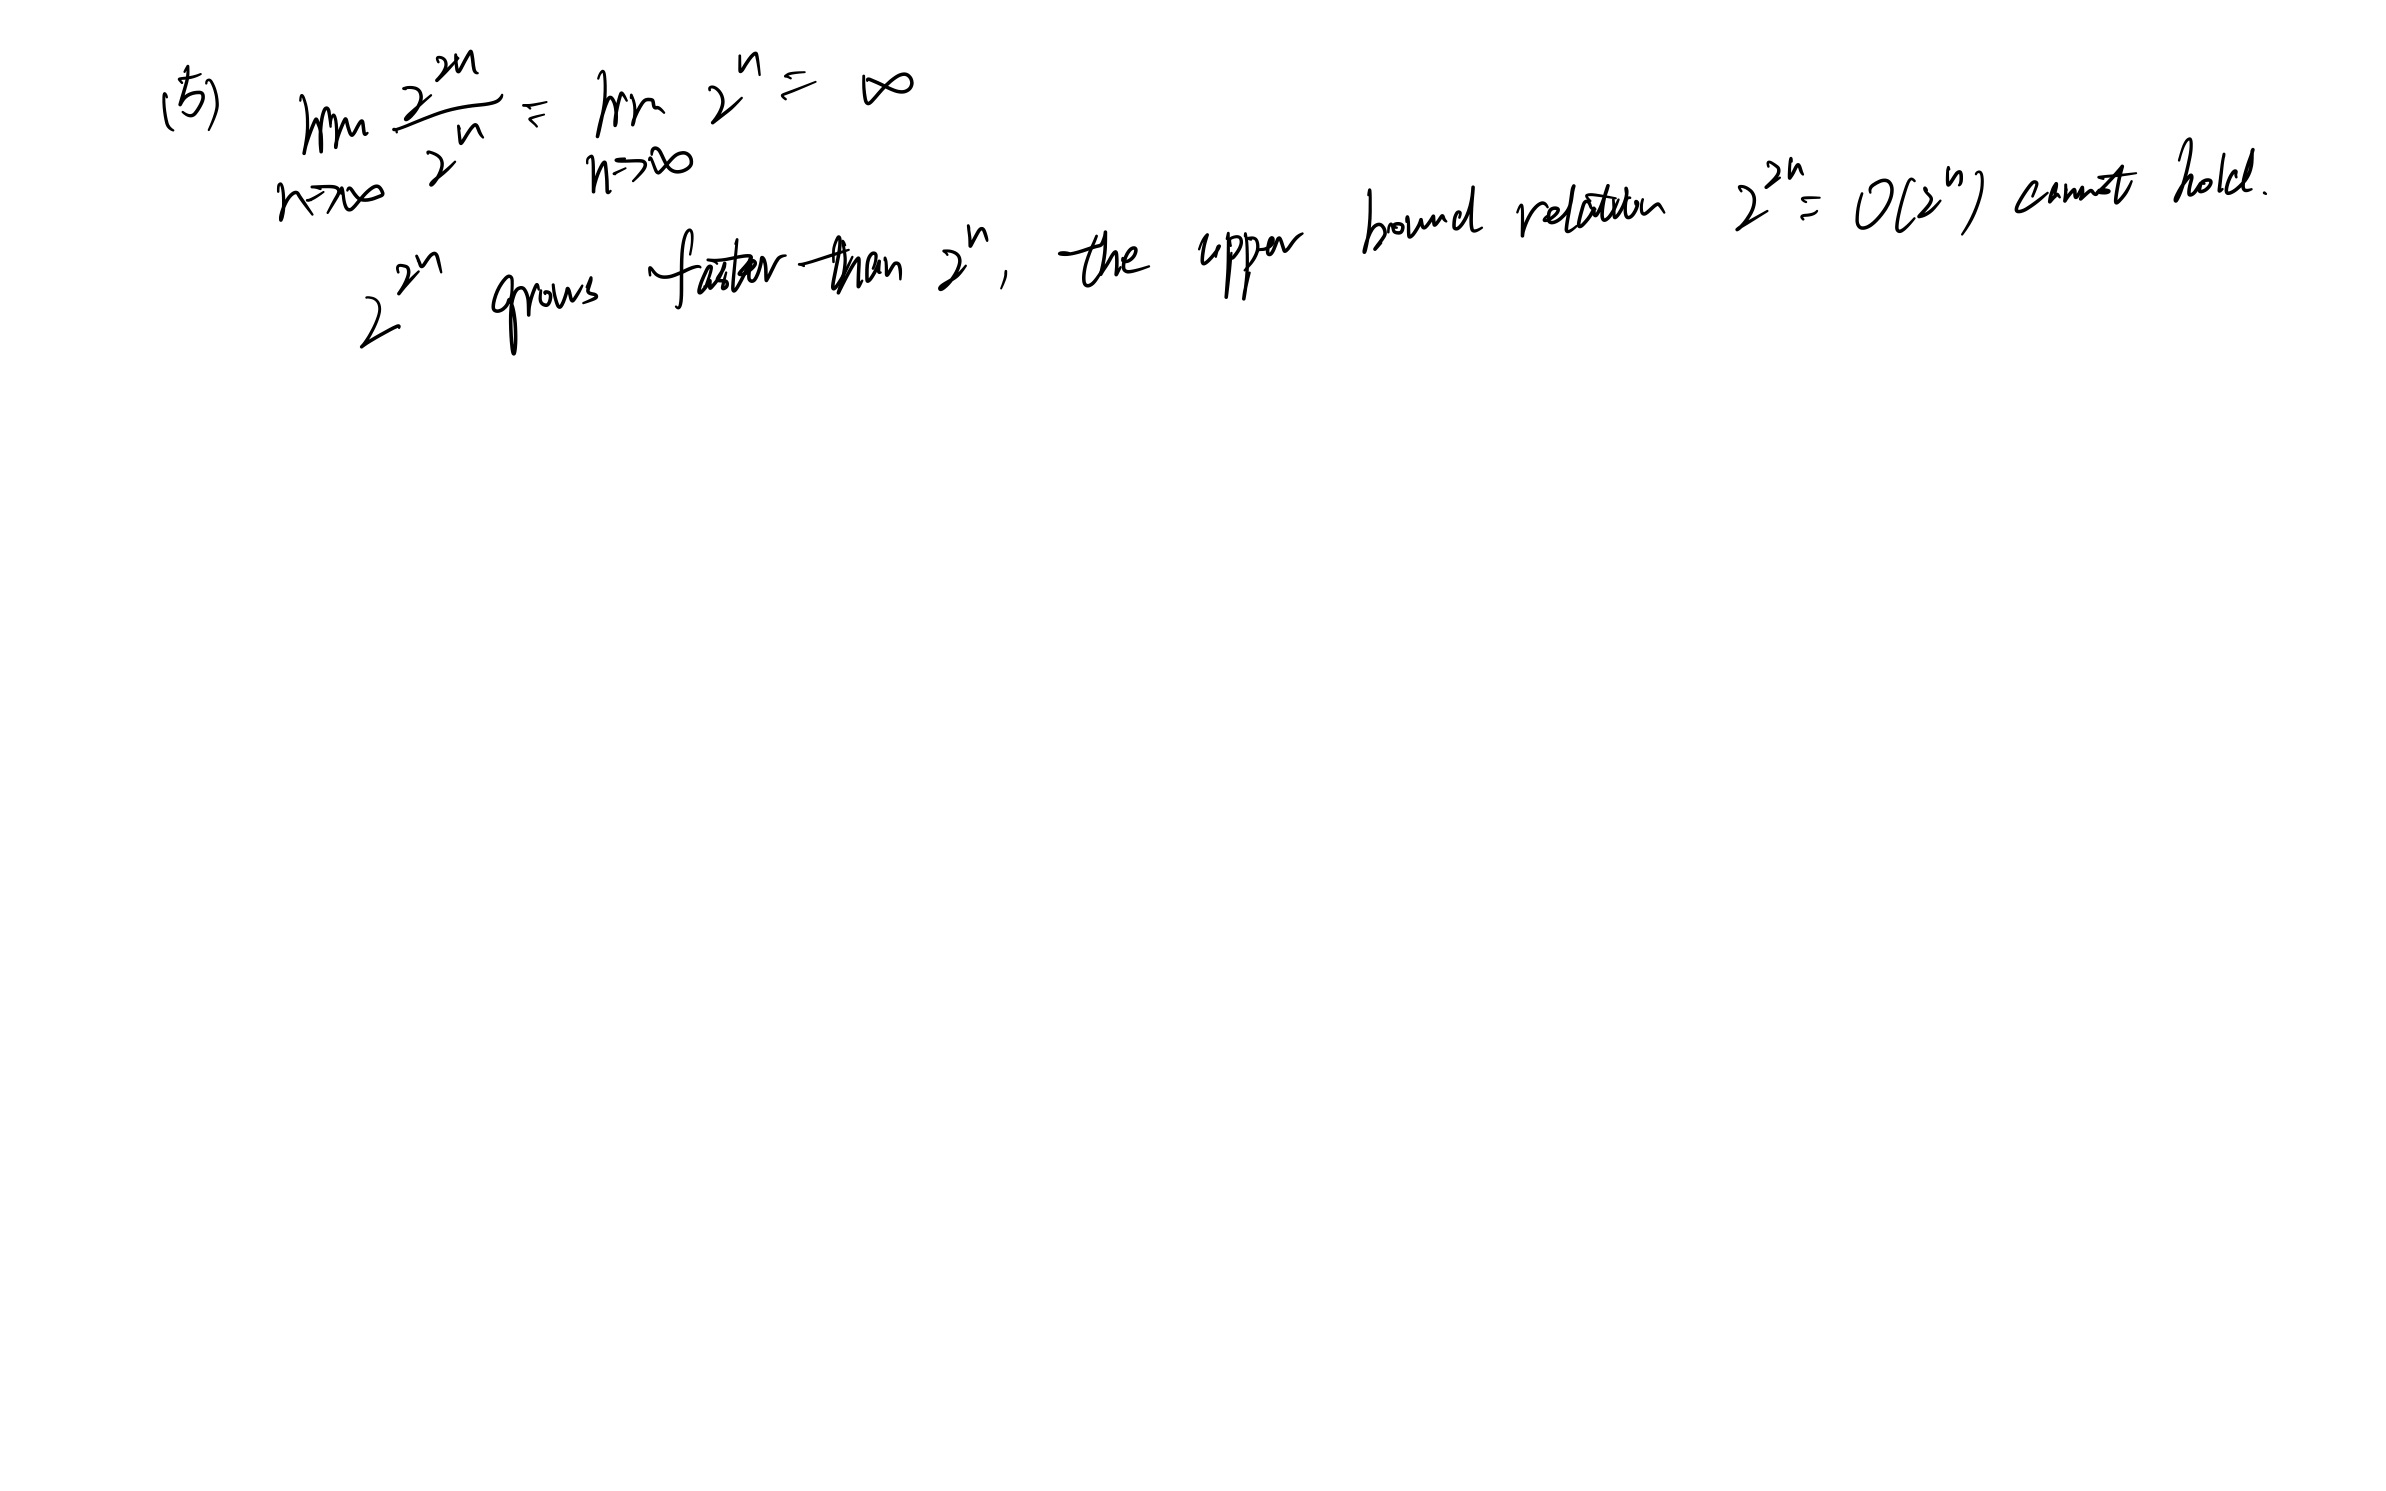
\includegraphics[width=\linewidth]{../assets/3_4.jpg}
\end{figure}

\section*{4. Evaluation}

For the following code snippet:

\begin{lstlisting}
for i to n:
    j = 1
    while j < sqrt{n}:
        j = j + (2 * k)
\end{lstlisting}

Analysis of execution times for each line:

\begin{center}
  \begin{tabular}{||c c c||}
    \hline
    line number & cost  & times                    \\
    \hline
    1           & $c_1$ & n + 1                    \\
    \hline
    2           & $c_2$ & n                        \\
    \hline
    3           & $c_3$ & $\sum_{i=1}^n t_i$       \\
    \hline
    4           & $c_4$ & $\sum_{i=1}^n (t_i - 1)$ \\
    \hline
  \end{tabular}
\end{center}

where $t_i$ denotes that the number of times the while loop {\bf test} in line 3 is executed for that value of $i$.

$t_i$ is determined by $k$ and $n$:

\newcommand{\ceil}[1]{\lceil {#1} \rceil}

\[t_i = \ceil{\frac{\sqrt{n}-1}{2k}}\]

Calculating the worst-case running time:

\begin{align*}T(n) & = c_1(n+1) + c_2n + c3\sum_{i=1}^n t_i + c_4\sum_{i=1}^n (t_i - 1)                                                   \\
                   & = c_1(n+1) + c_2n + c3\sum_{i=1}^n \ceil{\frac{\sqrt{n}-1}{2k}} + c_4\sum_{i=1}^n (\ceil{\frac{\sqrt{n}-1}{2k}} - 1)
\end{align*}

The highest order is $\frac{n^{1.5}}{k}$.

\end{document}